\section{PDF Implementierung}
PDF ist eine vektorbasierte \gls{pdl} (Seitenbeschreibungssprache) und basiert auf dem PostScript-Format. Der \gls{mime} Typ von PDF heißt application/pdf. Die standardisierten \gls{mime}-Typen (media types) zeigen Art und Format von Dokumenten, Dateien oder einem Sortiment von Bytes an. Ein \gls{mime}-Typ besteht üblicherweise immer aus einem durch ein / getrennten Typ und Subtyp. Der Typ repräsentiert die generelle Kategorie des Datentyps und der Subtyp die exakte Datenart des übergeordneten Typs. Jeder Typ hat seine eigene Menge an Subtypen \cite{mime}. Eine \gls{pdl} beschreibt den Seitenaufbau in einem Ausgabeprogramm bzw. Ausgabegerät, z.B. Drucker. \gls{pdl}s können Seiten mit Vektoren beschreiben. Mittels der \gls{pdl} wird ein Datenstrom der zu druckenden Ausgabe erzeugt und an den Drucker gesendet. Der \gls{rip} eines Druckers wandelt die Bildschirmausgabe in die gerasterte Druckerausgabe um. Viele APIs der Hardwareabstraktionsschicht im Computer wie GDI oder OpenGL können in \gls{pdl} ausgeben. Speichert ein Satzprogramm den Seitenbeschreibungscode eines Dokuments in einer Datei, muss der Drucker die \gls{pdl} nicht selbst verarbeiten. Zudem stellen \gls{pdl}s eine Schnittstelle zum Quellcode eines Dokuments bzw. zu Programmen, die Quellcode verwalten oder das Dokument formatieren können, dar. Die \gls{pdl} PDF erweitert die Funktionalität von PostScript um anklickbare Links (Hypertextfunktionalität), die die Navigation im Dokument erleichtern, und URLs, die sich automatisch im Browser öffnen \cite{wiki-pdl}.

\subsection{PostScript}
Sowohl die PostScript als auch PDF haben zum Ziel die Seiten eines Dokuments vollständig für die Ausgabe in der Druckvorstufe zu beschreiben. Die abwärtskompatible, stackorientierte, Turning-vollständige Hochsprache PostScript als \gls{pdl} wurde in den 1980er Jahren von Adobe erfunden \cite{adobe-postscript, wiki-postscript}. Hinzu wurden weitere PostScript-Technologien entwickelt, die aus der Programmiersprache PostScript, Grafik-, Textformatierungsanwendungen, Treibern und Abbildungssystemen bestehen. Die letzte Version ist PostScript 3 von 1997. Seine primäre Anwendung gemäß des Adobe Imaging Models findet sich in der Beschreibung von Textdarstellung, grafische Formen und Bildern auf gedruckten oder auf dem Bildschirm angezeigten Seiten. Dabei ist die Beschreibung des Dokuments geräteunabhängig und eine PostScript-Datei ist sequentiell organisiert. PostScript unterstützt u.a. beliebige, geometrische Formen, Zeichenoperationen in Graustufen, den RGB-, den druckbaren CMYK-Farbraum und das CIE-Normfarbsystem als Yxy-Farbraum. Vorinstallierte oder benutzerdefinierte Fonts, Digitalbilder jeglicher Auflösung – je nach Farbmodell – und ein allgemeines Koordinatensystem sind in PostScript ebenfalls implementiert. Der CMYK-Farbraum wird im Druck durch subtraktive Farbmischung mit den Farben Cyan, Magenta, Yellow und Key (Schwarz) verwendet. Einige Farben können nicht von CMYK reproduziert werden, dann spricht man von Sonderfarben.
\par
In PostScript wird eine Seite, die ein Koordinatensystem umspannt, als Grafik betrachtet, die verschiedene Grafikelemente enthalten kann. Dabei werden die Textzeichen eines Fonts, gemäß des Adobe Imaging Models, als graphische Formen betrachtet auf denen Grafikoperationen möglich sind. Das Koordinatensystem unterstützt alle linearen Transformationen, die auf jegliche Seitenelemente angewendet werden können. Die Seitenbeschreibung in PostScript kann auf jedem Gerät, welches einen PostScript-Interpreter implementiert, gerendert werden. In diesem Prozess wird die high-level PostScript-Beschreibung in low-level Rasterdatenformate für das jeweilige Gerät übersetzt. Jede PostScript-Datei muss durch einen \gls{rip} interpretiert werden und die Dateien können in ASCII vorliegen \cite{adobe-postscript}. Der PostScript-Interpreter als \gls{rip} rechnet die Benutzerkoordinaten in Gerätepixel um, wobei auch die technischen Eckdaten des jeweiligen Geräts mitberücksichtigt werden. Theoretisch kann derselbe PostScript-Code auf verschiedenen Endgeräten mit unterschiedlicher Auflösung eine mehr oder weniger identische Ausgabe erreichen. Den Interpreter gab es anfangs als Hardware-\gls{rip}, der allerdings nicht mehr zum Einsatz kommt. Heutzutage gibt es lediglich Software-\gls{rip}s, die von einem Betriebssystem kontrolliert werden und hardwareunabhängig arbeiten \cite{schneeberger}.

\subsection{Adobe Imaging Model}
PDF und die PostScript Programmiersprache haben das Adobe Imaging Model als Gemeinsamkeit. Es kann nahtlos zwischen PDF und PostScript konvertiert werden und beide erzielen das gleiche Ausgabeergebnis beim Druck. Dennoch fehlt PDF das general-purpose Framework der PostScript Programmiersprache. Stattdessen stellt ein PDF-Dokument eine statische Datenstruktur, optimiert für den random-access auf beliebigen Seiten, dar und enthält zusätzlich Seitennavigationsinformationen für interaktives Lesen. Im Kontrast dazu sind PostScript-Dateien seriell organisiert. Das high-level Imaging Model beschreibt die dargestellten Seitenelemente – Text, Geometrie, Vektorgrafiken – als abstrakte, graphische Elemente aus Vektorobjekten und Bézierkurven, anstatt als Pixeldefinitionen. Pfad-Objekte werden durch verbundene Punkte, Linien und Kurven mathematisch berechnet. Text-Objekte bilden eine eigene Datenstruktur (Fonts), die als Glyphen aus Pfad-Objekten bestehen. Bild-Objekte sind aus einzelnen Pixelwerten in einer rechteckigen Fläche aufgebaut und enthalten eine eindeutige Position im Rechteck und einen Farbwert. Die abstrakte Beschreibung graphischer Elemente macht das Imaging Model zu einem geräteunabhängigen Modell und es kann hochwertige Ausgaben auf vielen verschiedenen Druckern und Bildschirmen liefern. \cite{adobe-postscript}. Die Größe eines Pixels wird durch die Ausgabeauflösung des Rastergeräts bestimmt, die bei Monitoren zwischen 75 und 110 \gls{ppi} und bei Tintentstrahl- bzw. Laserdruckern zwischen 300 und 1400 \gls{ppi} liegt. Im Verlauf der Entwicklung wurde das Imaging Model ausschließlich für PDF um Transparenzen erweitert. Bei PostScript überschreibt das zuletzt gezeichnete Objekt alle darunterliegenden Objekte im Hintergrund \cite{schneeberger}. 

\subsection{Implementierung des Dateiformats}
PDF-Layouts können in linearar oder nicht linearer Form aufgebaut sein. Nicht lineare PDFs sind kompakter und werden mit größerer Verzögerung gerendert. Lineare PDFs sind für den Online-Bereich vorgesehen und werden auf die Festplatte in einer linearen Art und Weise gespeichert. Online-PDF-Viewer können die Datei bereits anzeigen, bevor sie komplett geladen wurde \cite{fileformat}. 

\subsubsection{Dateiformatstruktur}
PDF ist ein rein objektbasiertes Dateiformat und PDF-Dateien bestehen aus Sequenzen von 8-Bit-Binärdaten bzw. 7-Bit-ASCII \cite{schneeberger}. Die Struktur besteht im Wesentlichen aus 4 Komponenten. Zunächst spezifiziert der Header die Version der PDF-Spezifikation (signature) und den Charset Identifier \cite{ccc-pdf-secrets}. Ein Beispiel eines Headers ist in Abbildung \ref{fig:header1} gezeigt. Der Body enthält die Daten der Objekte, aus denen das Dokument besteht. Objekte im Body sind in einer komplizierten hierarchischen Struktur verknüpft. Zur Dateigrößenoptimierung werden komplexe Verbindungen zwischen den Daten hergestellt. Die Daten eines mehrfach vorkommenden Objektes müssen nur einmal gespeichert werden \cite{softx}. Jedes Objekt wird im Body mit obj und endobject umschlossen und jeder Stream mit stream und endstream \cite{schneeberger}. Die Beispielabbildung \ref{fig:body} visualisiert einen exemplarischen Body. Die Cross-Reference Table (Xref) deckt die Informationen über die Position der indirekten Objekte in der Datei ab. Liegt ein Verweis auf ein Objekt in der Xref, so kann es für andere Seiten wiederverwendet werden. In Xref sind alle Informationen für den random-access eingetragen. Neben Objekteinträgen können auch Cross-Reference-Streams hinterlegt werden. Xref ist der einzige Teil in PDF mit einem konstanten Format und kann aus mehreren Cross-Reference-Sections und Subsections, die jeweils Objekteinträgen für das incremental update enthalten, bestehen. Ein Objekteintrag ist wie folgt aufgebaut: Die ersten 10 Bytes für die Byteposition (Offset), ein Leerzeichen als 1 Byte zur Abtrennung, darauffolgende 5 Bytes für die eindeutige generation number und zuletzt eine ebenfalls durch ein Leerzeichen getrennte Markierung mit f oder n. F steht für free entry, d.h. gelöschtes Objekt und n für in use entry. Das erste Objekt in Xref hat eine generation number von 0 und wird nicht verwendet. Eine beispielhafte Xref wird in Abbildung \ref{fig:xref} dargestellt. Zuletzt definiert der Trailer die Startposition der Cross-Reference Table als Pointer startxref und die Startposition von speziellen Objekten im Body \cite{ccc-break-pdf}.  Außerdem enthält der Trailer die ID der PDF-Datei, einen Size Entry, Metadaten und eine Referenz zum /Root Objekt (Katalog) im Body. Abschließend markiert \%\%EOF das Dateiende \cite{ccc-break-pdf, ccc-pdf-secrets}. Ein Trailerbeispiel sind in Abbildung \ref{fig:trailer2} dargestellt. Beim incremental update wird am Ende des Original-Trailers ein Body-Update, eine neue Xref-Section und ein updated Trailer der Datei hinzugefügt. In der neuen Version der Xref-Section werden alle Objekte aufgeführt, die gelöscht, geändert oder ersetzt wurden. Der updated Trailer umfasst alle Änderungen bezüglich des originalen Trailers \cite{schneeberger}. 

\begin{figure}[!htb]
	\centering
	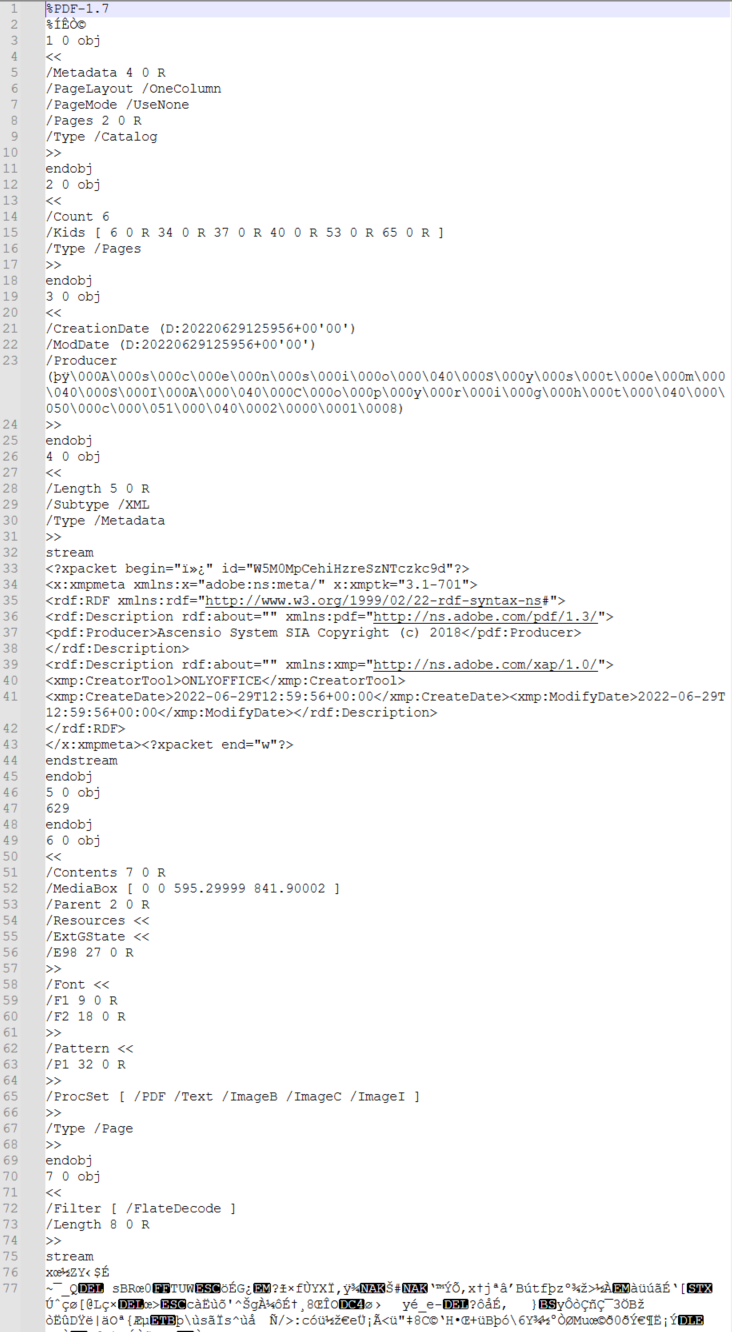
\includegraphics[width=0.8\textwidth]{"images/pdf_header2-notepad.png"}
	\caption{Header und Beginn eines Bodys des PDF-Dateiformats in Notepad++}
	\label{fig:header1}
\end{figure}

\begin{figure}[!htb]
	\centering
	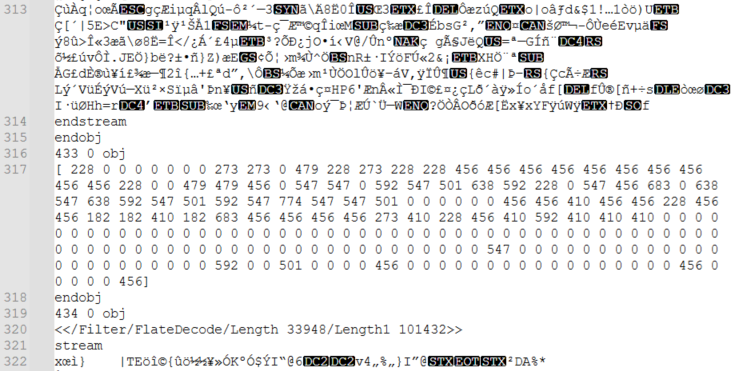
\includegraphics[width=0.8\textwidth]{"images/pdf_body2-notepad.png"}
	\caption{PDF Bodyauszug des PDF-Dateiformats in Notepad++}
	\label{fig:body}
\end{figure}

\begin{figure}[!htb]
	\centering
	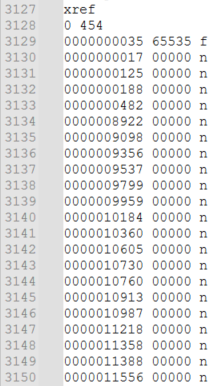
\includegraphics[width=0.3\textwidth]{"images/pdf_xref_start-notepad.png"}
	\caption{PDF Xref des PDF-Dateiformats in Notepad++}
	\label{fig:xref}
\end{figure}

\begin{figure}[!htb]
	\centering
	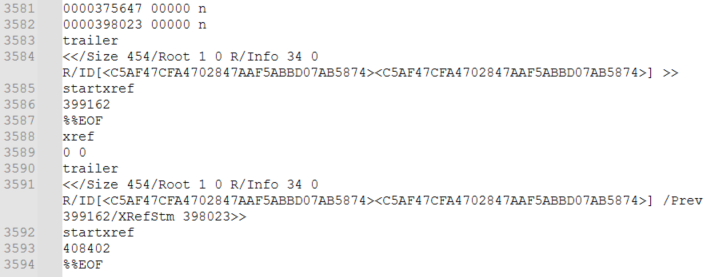
\includegraphics[width=0.8\textwidth]{"images/pdf_trailer2-notepad.png"}
	\caption{Ende einer Xref und Trailer des PDF-Dateiformats in Notepad++}
	\label{fig:trailer2}
\end{figure}

\subsubsection{PDF-Objekte und Operatoren}
Seitenobjekte und die meisten PDF-Strukturen sind gerichtete, azyklische Graphen \cite{ccc-wtf-pdf}. PDF-Objekte können in den folgenden Typen vorliegen: Booleans, Integers oder reelle Zahlen, Strings, Namen beginnend mit einem /, Arrays, Dictionaries, Streams, Null-Objekte oder Kommentare mit einem vorangestellten \%. Strings können als <Length> <string> oder <string> <terminating symbol> definiert werden. Dictionary Objekte sind als Objektpaare, genannt Entries, implementiert. Aktionen werden beispielsweise als Entries gespeichert \cite{ccc-badpdf}. Text in AcroForms sind Stream-Objekte. In Streams können jegliche Objekte gespeichert werden und werden nicht interpretiert. Die Objekte in Streams können Referenzen auf andere Objekte, vor allem Seiten, enthalten \cite{ccc-break-pdf}. Auf diese Art und Weise können Objekte gruppiert werden, wodurch eine bessere Komprimierung, insbesondere bei Linien, erreicht wird \cite{schneeberger}. Spezialisierte Operatoren können eine Datenstruktur, genannt graphics state, manipulieren. Graphics state fungiert als globales Framework. Es enthält die aktuelle Transformationsmatrix (CTM), welche die Benutzerortskoordinaten in Ausgabegerätekoordinaten mappt, die aktuelle Farbe, den aktuellen Clipping-Pfad und andere Parameter, die implizite Operanden von Zeichenoperatoren sind. Weitere Operatoren sind Pfaderstellungs-, Pfadzeichen- und Textoperatoren. Für den Dokumentenaustausch werden marked-content Operatoren verwendet \cite{fileformat}. 

\subsubsection{Parsing im PDF-Viewer}
PDF-Viewer prozessieren PDF-Dateien im Prinzip vom Ende bis zum Anfang, d.h. vom Trailer zum Body \cite{ccc-break-pdf}. Beim Parsen wird zunächst die signature überprüft. Anschließend wird die Position von \%\%EOF und startxref ermittelt. Die Xref stellt die Offsets jedes Objektes zur Verfügung und der Trailer zeigt auf den /Root Entry des Root-Objekts. Nachfolgend werden alle Objekte geparst und überprüft, ob /Root den /Pages Entry, /Pages ein Seiten-Array und jede /Page eine Größe der /MediaBox besitzt, sowie /Contents als Stream-Objekt vorliegt und /Resources das /Font Dictionary Definiert. Zuletzt wird die Seite durch BeginText, Auswahl des Fonts, Bewegung des Cursors, Anzeigen des Strings und EndText gerendert \cite{ccc-pdf-secrets}. Referenzen werden nicht in parse time ausgewertet, sondern nur nach Verwendung \cite{ccc-wtf-pdf}. 

\subsubsection{PDF-Boxen}
Grundsätzlich besteht eine PDF-Datei aus 5 Seitenrahmen als Boxen für jede Seite. Diese Boxen werden weder gedruckt, noch standardmäßig angezeigt. Die äußerste und größte Box ist die MediaBox. Sie entspricht der physischen Größe des Mediums und dem Papierformat. Sie muss immer in einer PDF-Datei vorhanden sein und enthält auch alle Objekte, die über den Rand der Seitengröße hinausragen, wobei diese über die MediaBox gehen können. Innerhalb der MediaBox befindet sich als nächste Box die CropBox. Sie entsteht durch das Beschneiden der Seite und definiert den Ausschnitt zur Anzeige in Acrobat. Zusätzlich wird sie meist zum Platzieren von PDF-Dokumenten in anderen Programmen und zum Ausdrucken aus Acrobat verwendet. Beim Erstellen der PDF-Datei hat die CropBox die Größe der MediaBox und ist immer vorhanden. Eine Ebene darunter liegt die BleedBox. Sie definiert die Beschnittzugabe, die in der Praxis meist auf 3 mm gesetzt wird. Diese Beschnittzugabe wird in der Druckvorstufe verwendet, damit keine weißen Blitzer am Rand des beschnittenen Druckbogens sichtbar sind. Die optionale BleedBox sollte kleiner als die MediaBox sein. Druckmarken wie Passkreuze, Schnittmarken oder Farbbalken sollten immer außerhalb der BleedBox liegen. Die TrimBox steht für die finale Größe des gedruckten und zugeschnittenen Dokuments. Ein zu druckendes Dokument benötigt zwingend die im PDF-Dateiformat optionale TrimBox, deren Größe kleiner oder gleich der BleedBox und MediaBox sein sollte. Der Standardwert für die TrimBox ist die Größe der CropBox. Ganz innen im Boxmodell von PDF liegt die ArtBox. Sie stellt einen Rahmen um alle druckbaren Objekte dar und legt somit den Inhalt fest. Meist sind ArtBox und TrimBox von der Größe her identisch. Im Bezug auf PDF/X-Dateien darf nur entweder die ArtBox oder die TrimBox vorhanden sein. Da die ArtBox optional ist, dient sie vor allem in Ausschussprogrammen als default Box, falls keine TrimBox angelegt wurde. Die Abbildung \ref{fig:boxen} zeigt eine Grafik des verschachtelten Box-Modells der PDF-Boxen.

\begin{figure}[!htb]
	\centering
	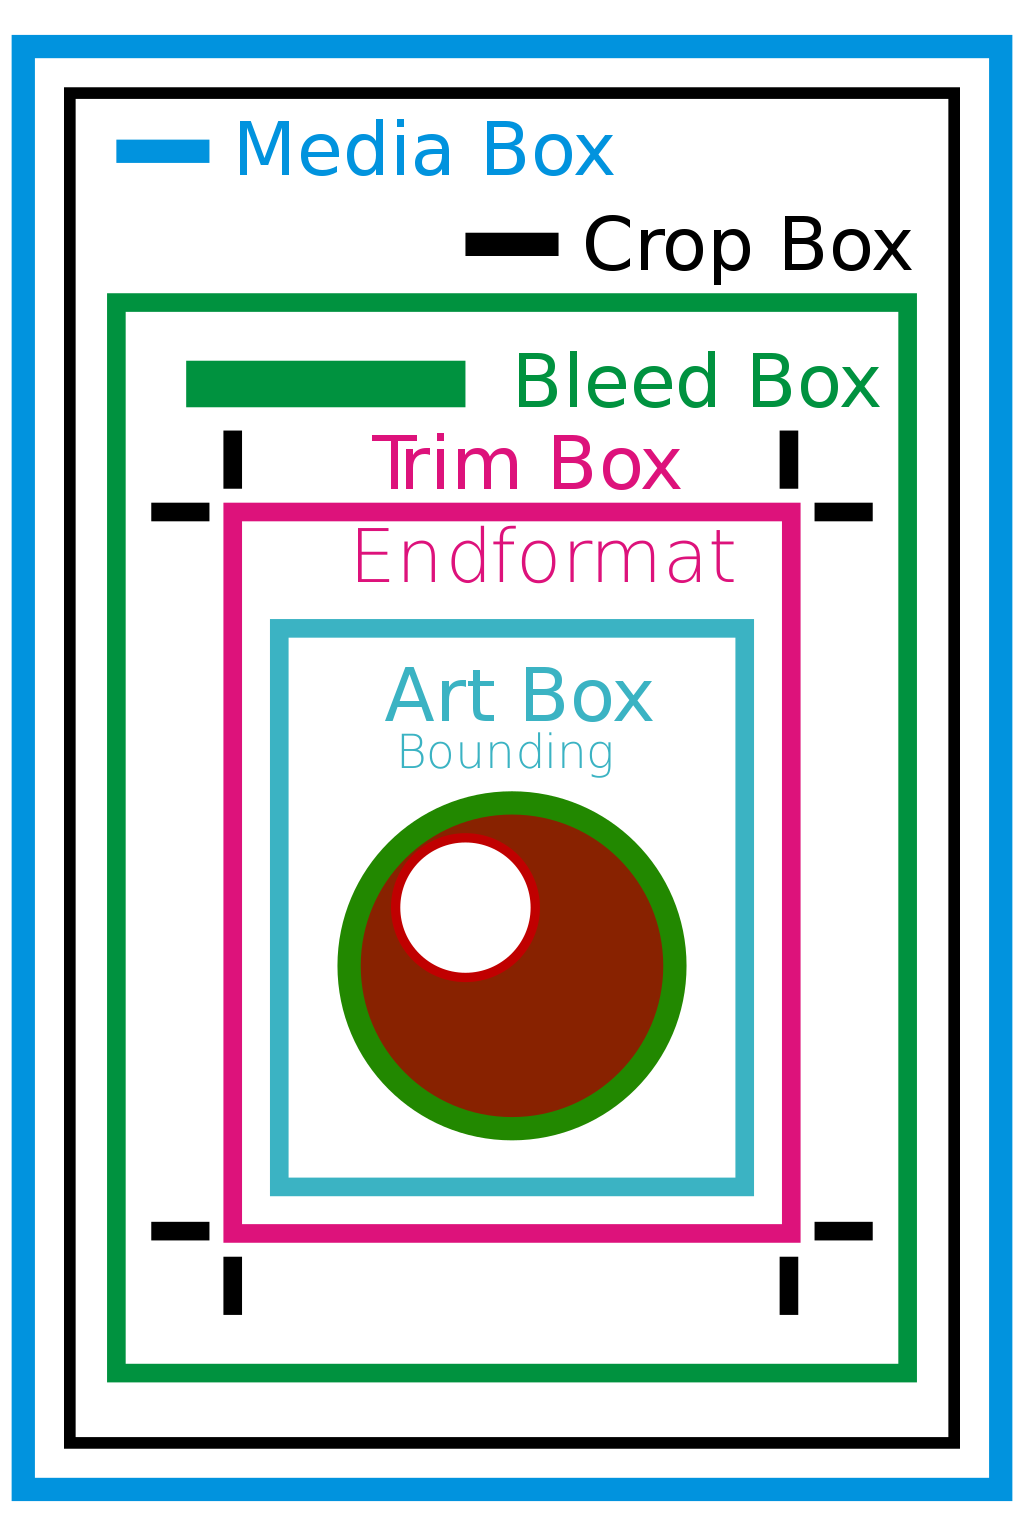
\includegraphics[width=0.5\textwidth]{"images/boxen-wiki-pdf-de.png"}
	\caption{Verschachtelte PDF-Boxen \cite{wiki-pdf-de}}
	\label{fig:boxen}
\end{figure}

\subsubsection{Seitenlayers}
Eine PDF-Datei besitzt 3 verschiedene layers, womit nicht die optional content layers gemeint sind. Zunächst enthält die content layer alle druckbaren Objekte, sprich Grafiken, Bilder und Texte. Elemente dieses layers können ausschließlich mit Acrobat Pro bearbeitet werden. Oberhalb der content layer positioniert sich die enhancement layer. In ihr sind Lesezeichen, Hyperlinks, Thumbnails, digitale Signaturen, Annotationen, Formularfelder und alle Multimedia-Elemente, wie Video und Audio, abgelegt. Die unsichtbare information layer umfasst alle Basisinformationen zu Schriftdaten, Formularfeldinhalten, Verschlüsselungsinformationen, Querverweistabellen und PDF-spezifische Informationen \cite{schneeberger}. 

\subsection{Implementierung von Fonts}
Schriften werden als Konturen (outlines) digital gespeichert und mit Instruktionen (hints) versehen, sodass sie generisch skaliert werden können. Fonts werden in PDF als eigenständige Dateien behandelt und die Darstellung wird durch einen speziellen Font-Interpreter bewerkstelligt. Innerhalb der Datei werden Fonts als Dictionary registriert, worin u.a. Fonttyp als Subtype, PostScript-Name, Verschlüsselung und Schriftklasse (für eine mögliche Ersatzschrift) abgelegt sind. Für jeden verwendeten Font wird ein Font-Descriptor in der Datei hinterlegt. PDF verarbeitet 2 Klassen von Fonttypen: Simple-Fonts und Composite-Fonts. Jede Glyphe im Dokument wird über einen Character Code prozessiert. Daraufhin erfolgt eine Zuordnung des Character Codes zum hinterlegten Encoding (Mapping). Zuletzt wird die Glyphe im aktuellen Font über die Glyphen-ID zum Zeichen der Glyphe aufgerufen. Folglich erzielt das Mapping des Codes und der Aufruf der Glyphe die benötigte Konturbeschreibung. Ein optionales Unicode-Mapping ToUnicode ist vonnöten, damit die Glyphen auch über Unicode verarbeitet werden können. Ist dieses Mapping nicht vorhanden, kann keine Textsuche und das Kopieren von Text stattfinden. Fehler im Mapping oder Modifikation von Schriften können zu falsche Ausgabebuchstaben, mangelnde Wiederverwendung und fehlerhafte Textkonvertierung führen.
\par
Eine Font-Einbettung kann als zweite Option als Object-Stream gespeichert werden bzw. können Fonts sich auf eine externe Referenz beziehen. Die Beschreibung von Glypen ist bei eingebetteten Schriften als Steam im Eintrag FontFile registriert. Schriftsubstitution findet immer dann statt, wenn der Character Code nicht mit der Encoding-Tabelle übereinstimmt. Häufig fehlen bestimmte Glypen im Font. Falls eine Outline-Beschreibung des Fonts zum Erstellungszeitpunkt nicht verfügbar ist, wird die Einbettung des Fonts verhindert. Dies kommt vor allem dann vor, wenn ein Font ein Schutzflag besitzt. Weitere Probleme bei der Schrifteinbettung sind u.a. Laufweitenfehler in Schriften, Fehler in der Buchstabenbeschreibung oder beim Cachen von Fonts. Zwecks der Schriftsubstitution müssen folgende allgemeine Informationen zu einem Font in der PDF-Datei gespeichert sein: Name der Schrift, Fontfamilie, Typ, Subtyp, Schriftstärke (font weight), Zeichenbreite, Laufweite, maximale Ausprägung der FontBox, Dickteninformationen, Positionsangaben über Versal- und x-Höhe und Winkel für Italic (kursiv). Diese Informationen sind selbst bei nicht eingebetteten Schriften vorhanden \cite{schneeberger}. 